\documentclass[12pt] {article}
\usepackage{times}
\usepackage[margin=1in,bottom=1in,top=0.6in]{geometry}

\usepackage{hhline}
\usepackage{subfig}
\usepackage{amsmath}
\usepackage{amsfonts}
\usepackage[inline,shortlabels]{enumitem}%enumerate with letters
\usepackage{mathrsfs} 
\usepackage[square,numbers]{natbib}
\usepackage{graphicx}
\bibliographystyle{unsrtnat}
\usepackage{float}
\usepackage[framed,numbered,autolinebreaks,useliterate]{../mcode}

\begin{document}

\title{EEC 289Q – Data Analytics for Computer Engineers \\ Homework 5}
\author{Ahmed Mahmoud}
\date{June, 7th 2018} 

\maketitle




%============Table========
%\begin{table}[tbh]
% \centering    
%\begin{tabular}{ |p{4cm}|| p{2cm}|p{2cm}|p{2cm}|p{2cm}|}
% \hline
% & Processor 1 &  Processor 2  & Processor 3 & Processor 4\\ \hhline{|=|=|=|=|=|}
% \hline
% Performance          &$1.08$        &$1.425$       &\textbf{1.52}  &   \\
% \hline
%\end{tabular} 
%\caption{Metric table for the four processors}
%   \label{tab:metric}
%\end{table} 
%============Figure========
%\begin{figure}[!tbh]
%\centering        
%   \subfloat {\includegraphics[width=0.65\textwidth]{fig2_4.png}}
%   \caption{ }
%   \label{fig:fig}
%\end{figure}


\section*{PCA Whitening:} 
The following listing shows our code for PCA, PCA whitening and ZCA whitening implementation applied to MNIST data set.
\begin{lstlisting}
%% Step 0a: Load data
clear;
close all;
addpath(genpath('../common'))
x = loadMNISTImages('../common/train-images-idx3-ubyte');
figure('name','Raw images');
randsel = randi(size(x,2),200,1);
display_network(x(:,randsel));
%%================================================================
%% Step 0b: Zero-mean the data (by row)
%%% YOUR CODE HERE %%%
avg = mean(x, 1); 
x = x - repmat(avg, size(x, 1), 1);
%%================================================================
%% Step 1a: Implement PCA to obtain xRot
%%% YOUR CODE HERE %%%
 sigma = x * x' / size(x, 2);
 [U,S,V] = svd(sigma);
 xRot = U'*x;
%%================================================================
%% Step 1b: Check your implementation of PCA
%%% YOUR CODE HERE %%%
covar = xRot*xRot'/(size(xRot,2)-1);

% Visualise the covariance matrix. You should see a line across the
% diagonal against a blue background.
figure('name','Visualisation of covariance matrix');
imagesc(covar);
%%================================================================
%% Step 2: Find k, the number of components to retain
%%% YOUR CODE HERE %%%
S_diag = diag(S);
k = sum(cumsum(S_diag)/sum(S_diag)<=0.99);
%%================================================================
%% Step 3: Implement PCA with dimension reduction
%%% YOUR CODE HERE %%%
xHat = U*[V(:,1:k)'*x;zeros(size(x,1)-k,size(x,2))];

% Visualise the data, and compare it to the raw data
% You should observe that the raw and processed data are of comparable 
% For comparison, you may wish to generate a PCA reduced image which
% retains only 90% of the variance.

figure('name',['PCA processed images ',...
    sprintf('(%d / %d dimensions)', k, size(x, 1)),'']);
display_network(xHat(:,randsel));
figure('name','Raw images');
display_network(x(:,randsel));
%%================================================================
%% Step 4a: Implement PCA with whitening and regularisation
epsilon = 1e-1; 
%%% YOUR CODE HERE %%%
xPCAwhite = diag(1./sqrt(diag(S) + epsilon)) * xRot;

%% Step 4b: Check your implementation of PCA whitening 
%%% YOUR CODE HERE %%%
covar=xPCAwhite*xPCAwhite'/size(xPCAwhite,2);

% Visualise the covariance matrix. You should see a red line across the
% diagonal against a blue background.
figure('name','Visualisation of covariance matrix');
imagesc(covar);
%%================================================================
%% Step 5: Implement ZCA whitening
%%% YOUR CODE HERE %%%
xZCAWhite = U * xPCAwhite;

% Visualise the data, and compare it to the raw data.
% You should observe that the whitened images have enhanced edges.
figure('name','ZCA whitened images');
display_network(xZCAWhite(:,randsel));
figure('name','Raw images');
display_network(x(:,randsel));
\end{lstlisting}
\newpage
Figure~\ref{fig:fig} shows the series of images produces by the code for an example image from the input data set. 
\begin{figure}[!tbh]
\centering        
   \subfloat [Raw input] {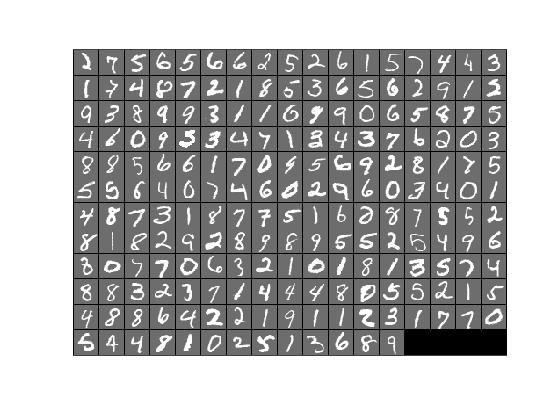
\includegraphics[width=0.3\textwidth]{raw_data.jpg}}
   \subfloat [$xRot$ covariance  Matrix] {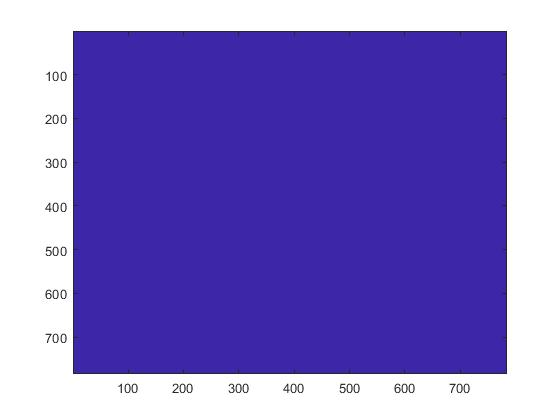
\includegraphics[width=0.3\textwidth]{covar_xrot.jpg}}
   \subfloat [PCA whitened (99\% variance)]{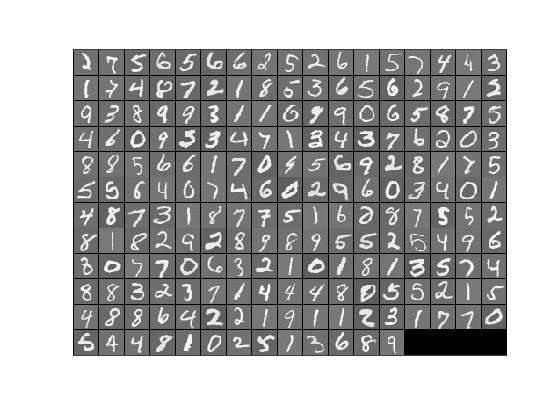
\includegraphics[width=0.3\textwidth]{PCA.jpg}}
   
   \subfloat [Covariance for PCA whitening with regularization]{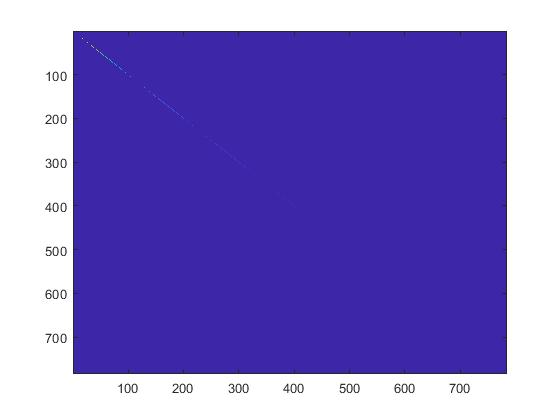
\includegraphics[width=0.3\textwidth]{covar_xPCAwhite.jpg}}
   \subfloat [ZCA whitened] {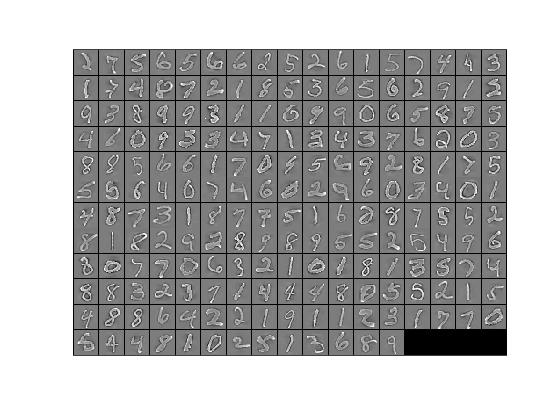
\includegraphics[width=0.3\textwidth]{xZCAwhite.jpg}}
   
   \caption{Showing the progress of the code on a single image from the input dataset. }
   \label{fig:fig}
\end{figure}

\end{document} 














































